
\documentclass[8pt]{article}
%	options include 12pt or 11pt or 10pt
%	classes include article, report, book, letter, thesis

\usepackage[a4paper,bindingoffset=0.2in,%
            left=0.4in,right=0.6in,top=0.2in,bottom=0.4in,%
            footskip=.15in]{geometry}
            
\usepackage[T1]{fontenc}
\usepackage[polish]{babel}
\usepackage[utf8]{inputenc}
\usepackage{lmodern}
\selectlanguage{polish}
\usepackage{blindtext}
\usepackage{pgfplots}
\usepackage{graphicx}


\title{Algorytmy numeryczne}
\author{Zadanie 3 \\ Tomasz Adamczyk | Aleksander Kosma\\243217 | 238193\\grupa 1 tester-programista}
\date{13 Grudzień 2017}

\begin{document}
\maketitle 

\section*{Informacje wstępne}
Większość testów została przeprowadzona dla danych wejściowych:\\

\begin{center}
\begin{tabular}{  | c | c | c | }
  \hline
  rozmiar planszy & ilość grzybów & wartości kostki \\\hline
  7 &4& -4 -3 -2 -1 0 1 2 3 4\\\hline
   pozycje graczy & pozycje grzybów & prawdopodobieństwo kostki \\\hline
   3 4& 1 2 5 6& 1 1 1 1 1 1 1 1 1\\\hline
  \hline
\end{tabular} 
\end{center}

Weryfikacja poprawnego działania metody Monte Carlo. Im więcej iteracji symulacji gry, tym wynik staje się precyzyjniejszy. W tym przypadku, wynik powinien zbiegać do wartości 0,6(wartość obliczona ręcznie).
\begin{center}
 \makebox[\textwidth]{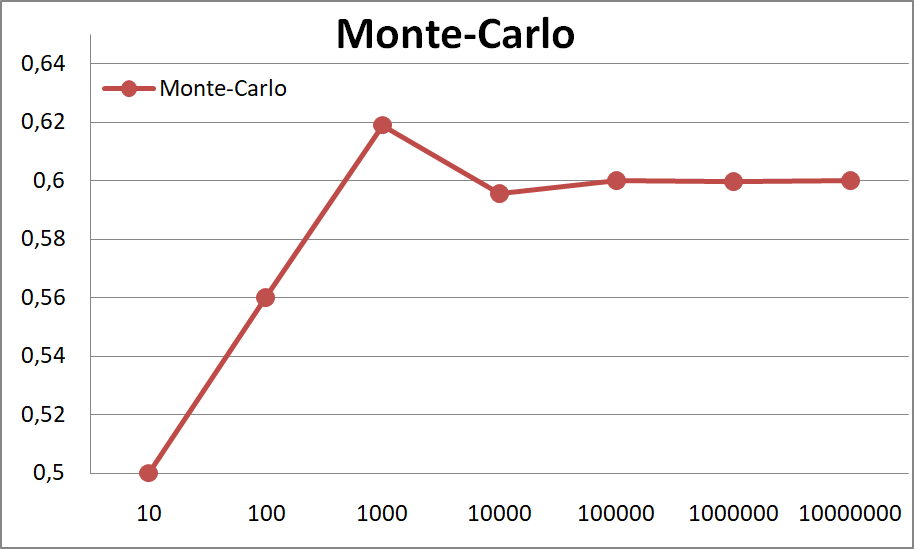
\includegraphics[width=9.5cm,height=5cm]{monte.png}}
\end{center}

\section*{Implementacja metod iteracyjnych}
W pierwszej części sprawozdania zbadamy poprawność metod iteracyjnych do rozwiązywania układów liniowych. Wyniki metod porównamy z wynikami z Eigen metodą Gaussa.\\ Lewy wykres prezentuje różnicę wyniku z metod iteracyjnych i wyniku Eigena. Widać że wyniki te wraz ze wzrostem liczby iteracji zbiegają do zera. Seidel już w około 130 iteracji osiągnął wartość równą Eigenowi. Jacobie potrzebował do tego  ponad 250 iteracji. Te wyniki dowodzą, ze metody iteracyjne liczą równie precyzyjnie co metoda Gaussa.\\
Prawy wykres prezentuje czas potrzebny do obliczenia wyniku dla podanych na osi poziomej iteracji.\\

\begin{center}
 \makebox[\textwidth]{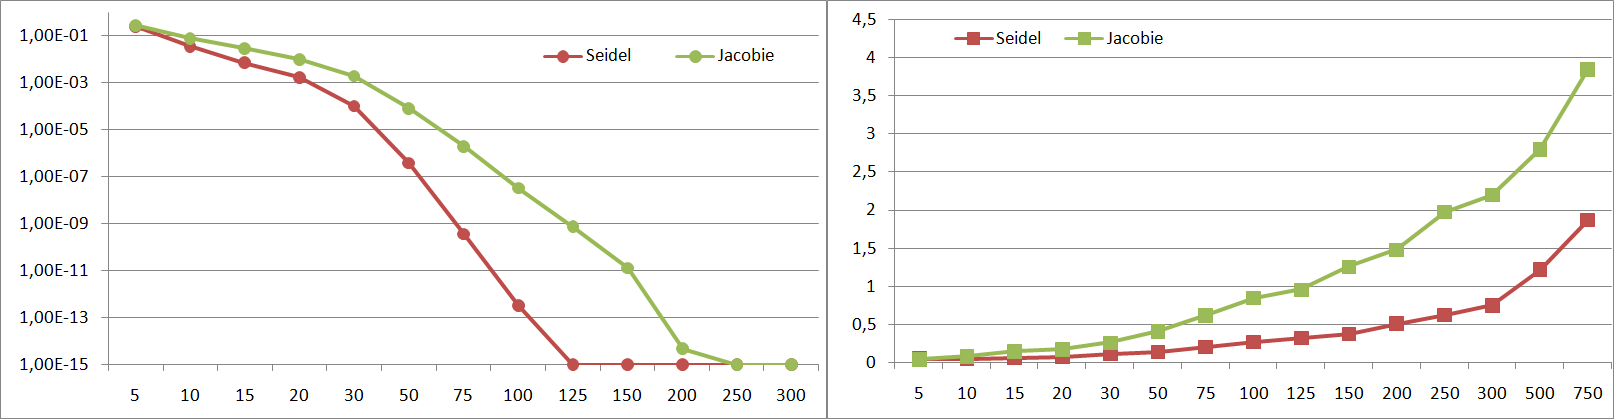
\includegraphics[width=20cm,height=6cm]{cmp2.png}}
\end{center}


\subsection*{Optymalna ilość iteracji w przypadku metod iteracyjnych}
Aby zoptymalizować czas potrzebny od wyliczenia wyniku przez metody iteracyjne, warto wiedzieć ile danych iteracji potrzebujemy. Za duża ilość iteracji może przeważyć na końcowych rezultatach i wnioskach.\\
Zastosowany został przez nas algorytm, wyliczający normę wektora poprzedniego i aktualnego. Jeśli ułamek tych norm jest mniejszy niż podany epsilon, kończymy kolejne iteracje. \\
Wykres pokazuje mniejszą potrzebę iteracji dla Gaussa-Seidela. Gdzie oś pionowa to ilość iteracji, a oś pozioma to rozmiar macierzy. Jacobie potrzebuje więcej iteracji, jak i szybciej przyspiesza z kolejnymi wymaganymi iteracjami. Więc wraz ze wzrostem macierzy potrzeba w obu przypadkach więcej iteracji.
\begin{center}
 \makebox[\textwidth]{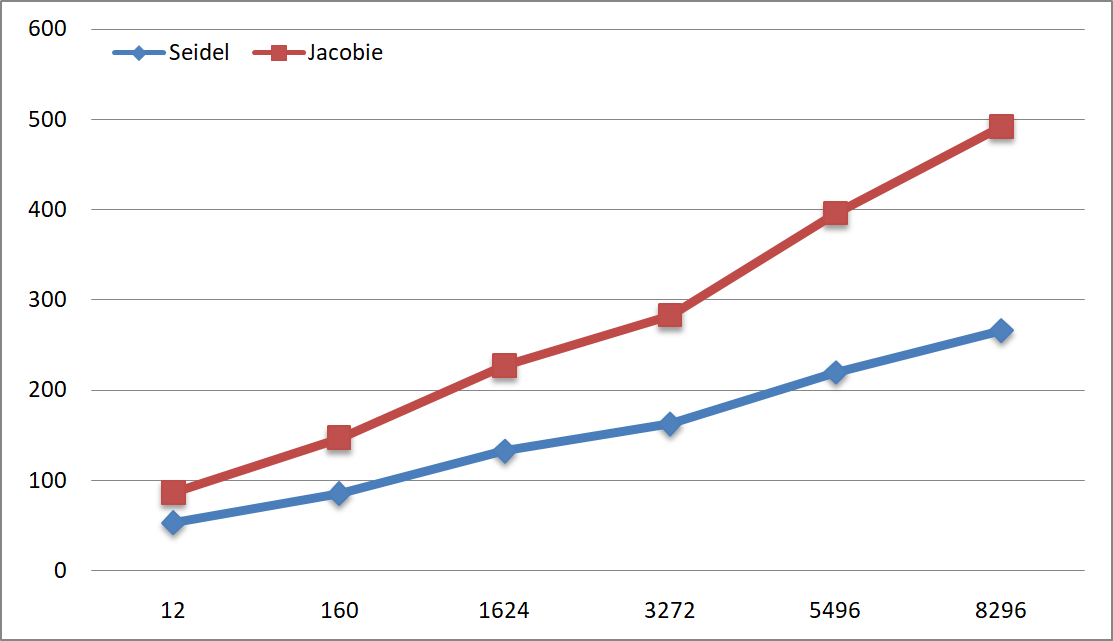
\includegraphics[width=12.5cm,height=7cm]{iteracje.png}}
\end{center}


\section*{Optymalny dobór metody w grze Grzybobranie}
Druga część opisuje wnioski, oparte o porównania wyników i czasu działania podanych metod:\\
-metoda Gaussa z częściowym wyborem elementu podstawowego\\
-metoda Gaussa z częściowym wyborem elementu podstawowego z optymalizacją dla macierzy rzadkich\\
-metoda iteracyjna Gaussa-Seidela\\
-metoda iteracyjna Jacobiego\\
-metoda z biblioteki Eigen partialPivLu, z częściowym wyborem elementu podstawowego\\
-metoda z biblioteki Eigen SparseLU, z częściowym wyborem przy użyciu macierzy rzadkich\\
\\
Poniższy wykres prezentuje czas potrzebny do rozwiązania równania, gdzie  oś pionowa to czas liczony w sekundach, oś pozioma rozmiar macierzy. Eigen sprase ma miażdżącą przewagę nad  wymienioną resztą. Z pośród podanych najlepiej korzystać z tej metody. Jedynym jej mankamentem jest potrzeba dostarczenia wektora z informacją o ilości wartości miejsc niezerowych w kolumnach. Trzeba jednak mieć na uwadze metody Seidela i Jacobiego w wersjach sparse, które mogą okazać się lepsze od wspominanego Eigena sparse. Dlatego nie można stwierdzić czy Eigen sparse jest najlepszą metodą z nam znanych.
\begin{center}
 \makebox[\textwidth]{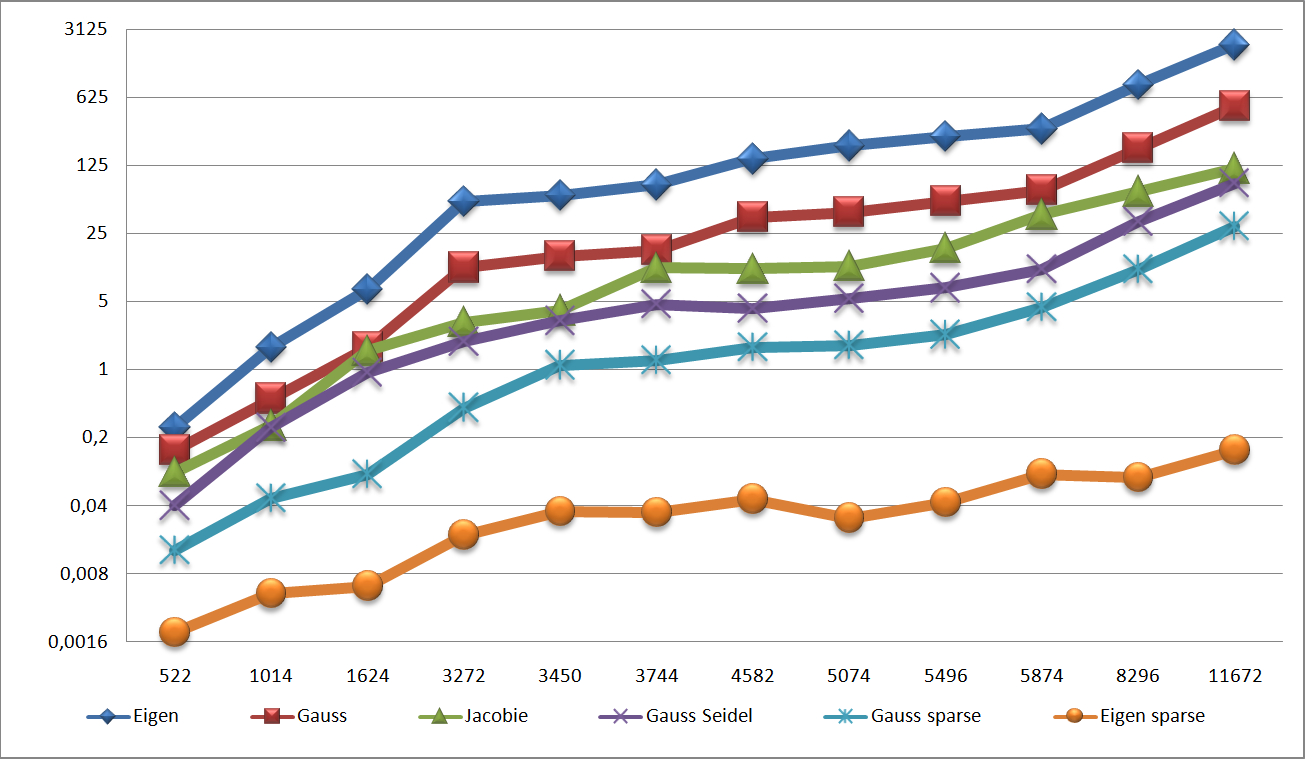
\includegraphics[width=16cm,height=9cm]{times.png}}
\end{center}
Precyzja wyników obliczona przez każdą z powyższych metod była praktycznie ta sama. W lwiej części sytuacji wyniki pokrywały się idealnie. Ma to związek z bardzo małą ilością wartości niezerowych wiec i operacji matematycznych. W konsekwencji strata precyzji nie jest zauważalna. Prawdopodobnie wraz ze wzrostem macierzy, mogłyby się pojawić pewne różnice w wynikach.\\

Treść zadania zakładała również kostkę, która ma dowolny rozkład wartości i ich prawdopodobieństw. Dane te mają jedynie wpływ na końcowy rezultat. Przez nieparzystą ilość pól na mapie, i rozmiar kostki, każde pole jest osiągalne dla obu graczy. Koniec końców możliwości rozegrania partii jest taka sama. Dlatego ciężko odnotować tu coś ciekawego i zostało to pominięte w sprawozdaniu.

Obliczenia wraz ze wzrostem rozmiaru macierzy były liczone od 10 do 2 próbek. Zazwyczaj tyle wystarczało by zauważyć tendencje. Wynik metody Monte Carlo do weryfikacji wyników, był obliczany każdorazowo dla miliona próbek.\\
\\
\begin{tabular}{ | p{8.2cm} | p{8.2cm} | }
  \hline
  \multicolumn{2}{|c|}{Podział obowiązków} \\
  \hline
  \multicolumn{1}{|c|}{\textbf{Aleksander Kosma} }& \multicolumn{1}{|c|}{\textbf{Tomasz Adamczyk}} \\
  \hline
  -Implementacja Monte Carlo & -Implementacja metod iteracyjnych \\\hline
   -Iteracyjne generowanie układu równań & -Ustalenie i implementacja warunków wygranej \\\hline
    -Szukanie gry bliskiej 50\% & -Wprowadzanie układu równań do macierzy \\\hline
  -Optymalizacja metod iteracyjnych i Gaussa & -Generowanie wyniku poprzez bibliotekę Eigen\\\hline
  -Testy i generowanie wyników & -Napisanie skryptów do generowania wyników \\\hline
  -Obróbka wyników, wykresy i opracowanie & - \\\hline
  
  \hline
\end{tabular}

\subsection*{Dodatkowo}

W momencie kiedy chcemy osiągnąć wynik jak najbardziej zbliżony do 50\% szans na wygraną, naszą intencją jest wydłużanie i  odwlekanie wygranej przez któregoś z graczy. W tym celu należy:\\
$\bullet$  \quad pozbyć się grzybów. Grzyby są ścieżką na skróty do wygrania. Określona ilość grzybów w rozgrywce, zdobyta wcześniej, od razu premiuje nas wygraną.\\
$\bullet$  \quad zmniejszyć kostkę do najmniejszych przeskoków. Najbardziej optymalna wersja to kostka ze ściankami o wartościach \{-1, 0 ,1\}. Zero na kostce jest kolejną szansą dla przeciwnika by odwrócić losy rozgrywki.\\
$\bullet$  \quad prawdopodobieństwo kostki powinno być jak największe dla zera.  W momencie kiedy zero wypada najczęściej, dynamika rozgrywki spada. Dzięki temu, któremuś z graczy trudniej stworzyć sobie szybką przewagę. \\
$\bullet$  \quad Ostatnią zmienną na którą mamy wpływ to pozycje startowe graczy. Znów chcemy by opóźnić wygraną, więc stawiamy obu graczy możliwie daleko od mety.\\
Najlepszy uzyskany wynik:  \textbf{0.5000000034688313}\\
\begin{center}
dane wejściowe: \\

\begin{tabular}{  | c | c | c | c | }
  \hline
  rozmiar planszy &pozycje startowe& wartości kostki & prawdopodobieństwo \\\hline
   101 & 50, 51  & -1, 0, 1& 1, 100000, 1\\\hline
  \hline
\end{tabular} 
\end{center}

\end{document}